

\documentclass{article}
\usepackage{graphicx}
\usepackage{hyperref}


\title{Computer Vision Sprint 3 Status}
\date{12/3/15}
\author{Jon Dixon}

\begin{document}
	\maketitle
	\newpage
	
	\section{Introduction}
	The purpose of this report is to give a brief overview of the current status of the computer vision approach to landing. I've been playing around with some different ideas for how to do this, and have read a few papers, which will have links in this document.
	
	\section{Blob Detection Approach}
	The prototype 2 document located in the repository in the directory: \hfill\hfill\linebreak landingpad/Documents/Prototypes/Sprint\_2 gives details on the old code, so this will focus on progress made in sprint 3. For information on how to compile the old C code, see the document in that directory. \hfill\hfill\linebreak\linebreak
	After the work done in the computer vision class, we decided to move away from the three-blob approach, and use four colored circles. The hope is that this will allow us to detect four points, and compute an accurate homography matrix for orientation, range, etc... Below is an image of the current layout being used in testing and development.
	
	\begin{figure}[h]
		\centering
		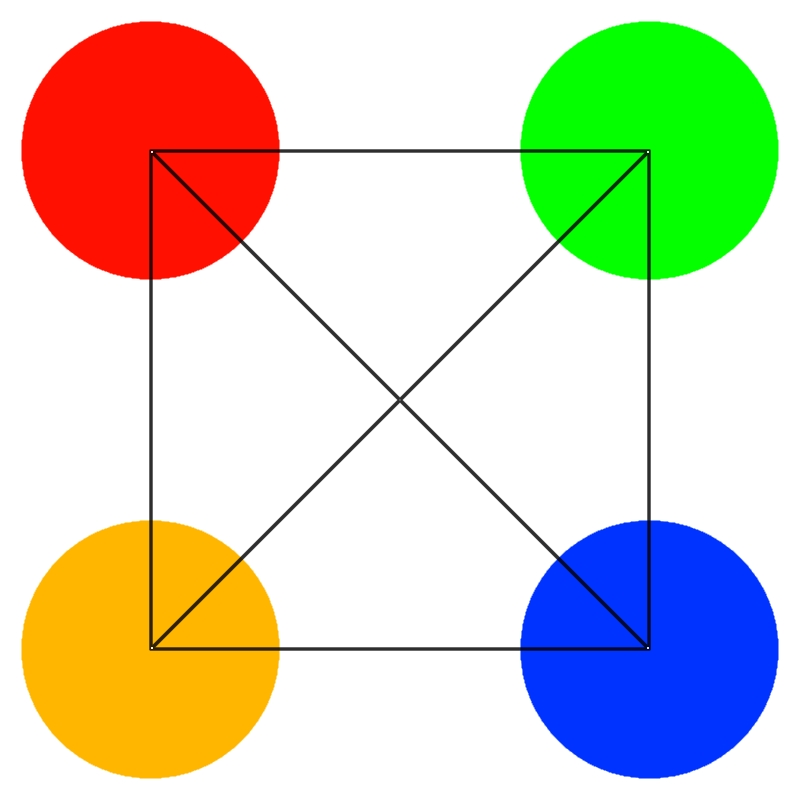
\includegraphics[width=0.5\textwidth]{landing_guide_small_x.jpg}
		\caption{Four-blob landing guide}
	\end{figure}
	
	The approach we've been messing with is to compute a homography matrix based on the four detected points, which would then be used to warp the image so that the blobs are essentially in a "square." The next step will be to use the homography matrix to calculate the angle of rotation, and translation. This will allow us to see how far the target is offset, and calculate the angle that we will need to yaw the quad.
	
	\section{Other possible approaches}
	While doing research for graduate seminar, I read a number of papers on the topic of autonomous landing that all had various approaches to pad target design, and actual landing algorithms. These approaches all ended up using similar methods of image preprocessing, using binarization and thresholding. The next step will be to attempt to apply these to our own target design to see if we are able to use a similar approach.\hfill\hfill\linebreak\linebreak
	At the same time, I have been working with learning OpenCV within python. One of the interesting things I discovered is the hough transform for circle detection. some preliminary testing seems to indicate that this will work relatively well for detecting circles, so I may play around with that some to see if there is anything useful I can come up with. Below is an image of the target above and some circles detected on it. One issue that I have had with this is there are a lot of false positives being detected, so if I play around with image preprocessing, I may be able to reduce the amount of these being detected.
	
		\begin{figure}[h]
			\centering
			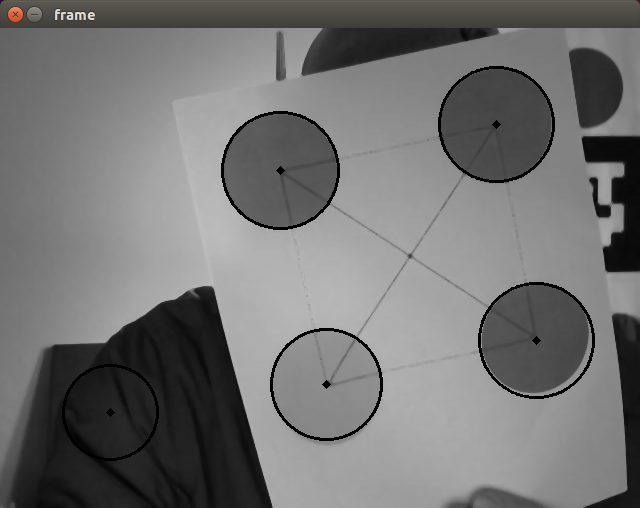
\includegraphics[width=0.5\textwidth]{circles.png}
			\caption{Hough detection on the target}
		\end{figure}
		
	Additionally, I am still interested in the possibility of using AR tags for this, so I will be looking into that in the future.
	
	\section{Next Steps}
	My plan now is to work to do more actual image processing to improve the reliability of any feature detection we will be doing. At the same time, I will be working to learn OpenCV, and find any useful functions that we can implement. In the meantime, I will be working in the github repository under the cv\_python branch, in the cv\_tracker directory.
	
	\section{Useful Reading}
	Here are links to the possibly useful papers on autonomous vehicle landing algorithms:\newline
	\href{http://citeseerx.ist.psu.edu/viewdoc/download?doi=10.1.1.24.7707&rep=rep1&type=pdf}{Paper with thresholding and corner detection}\newline
	\href{https://claraty.jpl.nasa.gov/man/overview/publications/related/03_montgomery_helicopter_icra.pdf}{Paper focusing on image thresholding}\newline
	\href{http://www.dis.uniroma1.it/lmarchetti/private/quadrotor/lange-vision-based-onboard-approach-landing-position-control-UAV-gps-denied-environments.pdf}{Interesting paper using concentric circles on landing pad}
	
\end{document}